% The two-stage scenario tree, and why a third stage is expensive.
%
% Single source for the diagram in optimization-private/lecture-notes/lectures/
% stochastic-programming-intro.tex, which \input's it via \figsrc. `make` also
% renders ../media/figures/scenario-tree.{png,svg} for the website, which draws
% this nowhere -- claude/figure_inventory.md, L8: "the scenario tree, the
% canonical figure for two-stage SP, is not drawn anywhere. TikZ job."
%
% LEFT  two stages: one here-and-now decision x, then the uncertainty resolves,
%       then one recourse decision y_s PER SCENARIO. The whole content of the
%       two-stage model is that x has no subscript and y does.
% RIGHT the same picture with one more stage, to show the branching is
%       multiplicative: 3 -> 9 leaves, and the farmer's 3-scenario extensive
%       form would become a 9-scenario one.
%
% Greyscale: nothing is encoded by hue. The stage-1 node is deliberately filled
% GREY rather than a pale blue -- a second blue tint blends with the black
% strokes under antialiasing and scripts/check_greyscale.py (image mode) then
% reports those blends as series that collapse in print. Grey removes the
% near-pair entirely and costs nothing, because shape already carries the
% distinction.
%
% Nothing is encoded by hue. Stage 1 is a filled node, stage 2 an
% open one, stage 3 a small dot; the probabilities are written on the edges;
% the stage boundary is a labelled dashed rule. Every distinction is shape or
% text, so the figure is identical in black and white.
%
%
% ⚠ DRAWN IN BLACK AND GREY, NOT BLUE -- and that is a considered decision, not
% an oversight. scripts/check_greyscale.py runs on the RENDERED IMAGE. A thin
% coloured stroke antialiases into a family of intermediate tones, so a blue
% diagram reports four or five "data colours" that are nothing but edge pixels,
% several of which collapse to the same grey and FAIL the gate. Measured on
% this figure: five data colours, four failing pairs. Black and grey blend only
% into greys, which the checker recognises as monochrome and passes outright.
% All three pre-existing tenants of this directory -- pendulum,
% farmer-crop-allocation, reactor-selection -- are black line art and all three
% PASS, so this is the house precedent rather than a new rule. Nothing is lost
% here: the contrast was already carried by solid-vs-dashed and by the two
% written captions, which is what "redundant encoding" means.

% `positioning' is loaded HERE rather than in the course-pack preamble so this
% file is self-contained: the same source is \input by the lecture and built
% standalone by figures/Makefile, and only the standalone wrapper happened to
% load the library. Without it `left=3pt of x' is a fatal PGF math error and
% the WHOLE course pack fails to produce a PDF. \usetikzlibrary is idempotent,
% so loading it twice is harmless.
\usetikzlibrary{positioning}

\begin{tikzpicture}[>=stealth, font=\small,
    root/.style={circle, draw=black, fill=gray!35, minimum size=6.5mm,
                 inner sep=0pt},
    leaf/.style={circle, draw=black, fill=white, minimum size=6.5mm,
                 inner sep=0pt},
    twig/.style={circle, draw=black, fill=black, minimum size=2.6mm,
                 inner sep=0pt},
    br/.style={->, thick, draw=black},
    plab/.style={font=\scriptsize, inner sep=1.5pt}]

% ===================== LEFT: two stages =====================
  \node[root] (x) at (0,0) {};
  \node[left=3pt of x, align=right] {$x$\\[-2pt]\scriptsize here-and-now};

  \foreach \i/\y/\p/\name in {1/1.55/{$p_1=\tfrac13$}/{$y_1$},
                              2/0.00/{$p_2=\tfrac13$}/{$y_2$},
                              3/-1.55/{$p_3=\tfrac13$}/{$y_3$}} {
    \node[leaf] (l\i) at (3.1,\y) {};
    \draw[br] (x) -- (l\i) node[plab, midway, above] {\p};
    \node[right=3pt of l\i] {\name};
  }

  % the stage boundary: everything left of it is decided before anything is known
  \draw[dashed, gray!80] (1.55,-2.35) -- (1.55,2.35);
  \node[gray!70, font=\scriptsize, align=center] at (1.55,-2.75)
    {yields\\observed};

  \node[font=\small\itshape] at (1.55,2.75) {two stages: 3 scenarios};

% ===================== RIGHT: three stages =====================
  \begin{scope}[xshift=7.9cm]
    \node[root] (X) at (0,0) {};

    \foreach \i/\y in {1/1.55, 2/0.00, 3/-1.55} {
      \node[leaf] (L\i) at (2.2,\y) {};
      \draw[br] (X) -- (L\i);
      \foreach \j/\d in {1/0.52, 2/0.0, 3/-0.52} {
        \node[twig] (T\i\j) at (4.3,{\y+\d}) {};
        \draw[br] (L\i) -- (T\i\j);
      }
    }

    \draw[dashed, gray!80] (1.1,-2.35) -- (1.1,2.35);
    \draw[dashed, gray!80] (3.2,-2.35) -- (3.2,2.35);
    \node[gray!70, font=\scriptsize] at (1.1,-2.75) {stage 2};
    \node[gray!70, font=\scriptsize] at (3.2,-2.75) {stage 3};

    \node[font=\small\itshape] at (2.2,2.75) {three stages: 9 scenarios};
  \end{scope}
\end{tikzpicture}
